%%%%%%%%%%%%%%%%%%%%%%%%%%%%%%%%%%%%%%%%%%%%%%%%%%%%%%%%%%%%%%%%%%%%%%%%%%%%%%%
% MOTIVATION
%%%%%%%%%%%%%%%%%%%%%%%%%%%%%%%%%%%%%%%%%%%%%%%%%%%%%%%%%%%%%%%%%%%%%%%%%%%%%%%
\def\no{\monoUpR{}{\textbf{No$_{\downarrow \downarrow}$}}{}{}}
\def\carnivores{\monoDownR{felines}{carnivores}{animal}{organism}}
\def\eat{\monoDownR{slurp}{eat}{consume}{}}
\def\animals{\monoDownR{chordate}{animals}{organism}{living thing}}

%%%%%%%%%%%%%%%%%%% 
% COMMON SENSE REASONING TEASER
%%%%%%%%%%%%%%%%%%%
\begin{frame}{Reasoning About Common Sense Facts}
\begin{tabular}{cc}
  \true{Kittens play with yarn} & \false{Kittens play with computers} \\
  \vspace{0.25cm} \\
  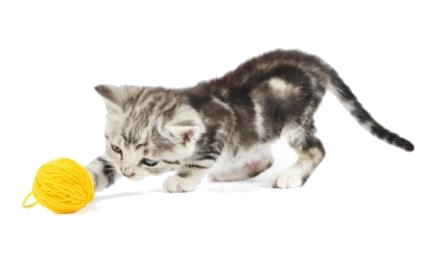
\includegraphics[width=5cm]{../img/yarn-cat.png} & \pause 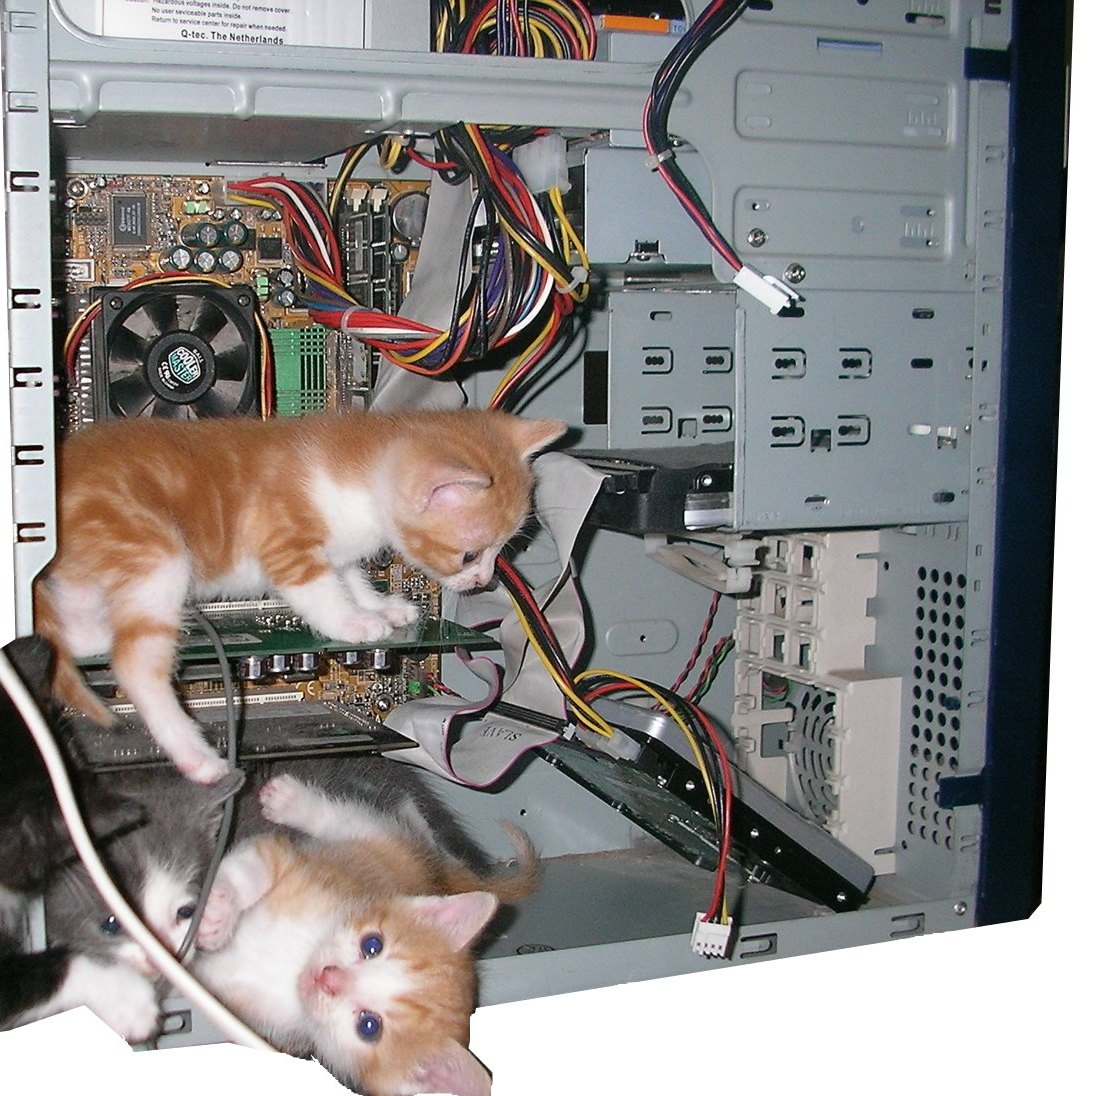
\includegraphics[width=5cm]{../img/computer-cat-cropped.jpg}
\end{tabular}
\end{frame}


%%%%%%%%%%%%%%%%%%% 
% COMMON SENSE REASONING NLP
%%%%%%%%%%%%%%%%%%%
\begin{frame}{Common Sense Reasoning for NLP}
\begin{center}
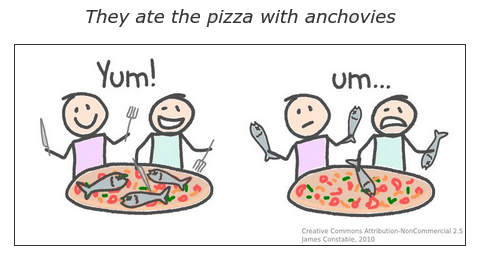
\includegraphics[width=8cm]{../img/ambiguity.png}
\end{center}
\end{frame}

%%%%%%%%%%%%%%%%%%% 
% TEASER
%%%%%%%%%%%%%%%%%%%
\begin{frame}{Start with a large knowledge base (270M facts)}
\begin{center}
  \hspace{0.8cm}
  
\includegraphics[height=2.2cm]{../img/database.png}
\end{center}
\end{frame}

\begin{frame}[noframenumbering]{Start with a large knowledge base (270M facts)}
\begin{center}
  \teaserManyPremises
\end{center}
\end{frame}

\begin{frame}[noframenumbering]{Infer new facts...}
\begin{center}
  \teaserBlindInferenceNaturalOrderBlind
\end{center}
\end{frame}

\begin{frame}[noframenumbering]{Infer new facts...}
\begin{center}
  \teaserBlindInferenceNaturalOrder
\end{center}
\pause
\begin{textblock*}{6.0cm}(6.5cm,5cm)
  \textcolor<1-1>{white}{$\uparrow$ Don't want to run inference \\ $~~$ over every fact!}
\end{textblock*}
\pause
\begin{textblock*}{6cm}(5.5cm,7.6cm)
  \textcolor<1-2>{white}{$\leftarrow$ Don't want to store all of these!}
\end{textblock*}
\end{frame}

\begin{frame}[noframenumbering]{Infer new facts...on demand from a query...}
\begin{center}
  \teaserBlindInference
\end{center}
\end{frame}

\begin{frame}[noframenumbering]{...Using text as the meaning representation...}
\begin{center}
  \teaserInference
\end{center}
\end{frame}

\begin{frame}[noframenumbering]{...Without aligning to any particular premise.}
\begin{center}
  \teaserFullDerivation
\end{center}
\end{frame}


%%%%%%%%%%%%%%%%%%% 
% INFERENCE IS SEARCH
%%%%%%%%%%%%%%%%%%%
\def\title{A Search Problem}
\begin{frame}{\title}
\begin{center}
  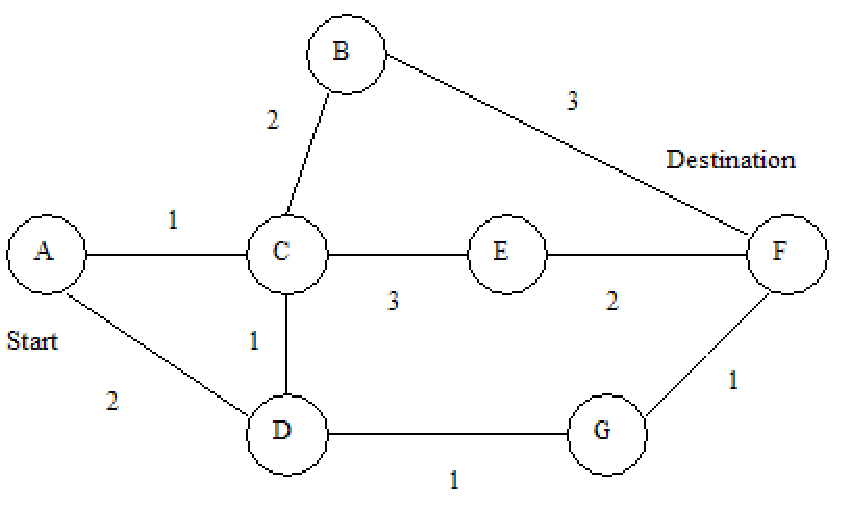
\includegraphics[width=5cm]{../img/dijkstras-graph.pdf}
\end{center}
\begin{tabular}{ll}
  \hh{Nodes} & $($ \w{fact}, truth maintained $\in\{\textrm{true}, \textrm{false}\})$ \\
  & \\
  \pause
  \hh{Start Node} & $($ \w{query fact}, \true{true} $)$ \\
  \hh{End Nodes}  & \w{any known fact} \\
  & \\
  \pause
  \hh{Edges} & Mutations of the current fact \\
  \hh{Edge Costs} & How ``wrong'' an inference step is (learned) \\
\end{tabular}
\end{frame}

%\input exampleSearch.tex

%%%%%%%%%%%%%%%%%%%%%%%%%%%%%%%%%%%%%%%%%%%%%%%%%%%%%%%%%%%%%%%%%%%%%%%%%%%%%%%
% NATURAL LOGIC
%%%%%%%%%%%%%%%%%%%%%%%%%%%%%%%%%%%%%%%%%%%%%%%%%%%%%%%%%%%%%%%%%%%%%%%%%%%%%%%

%%%%%%%%%%%%%%%%%%% 
% MUTATIONS ARE LOGIC
%%%%%%%%%%%%%%%%%%%
\begin{frame}{A Search Problem Over Valid Inferences}
\hh{Transitions (mutations) have to be precise:}
\vspace{2ex}

\begin{center}
\begin{tabular}{lll}
\w{\textbf{The} carnivores eat animals} & \textbf{$\vDash \lnot$} & \darkred{\textit{\textbf{No} carnivores eat animals}} \\
\w{\textbf{The} carnivores eat animals} & \textbf{$\vDash$}       & \darkgreen{\textit{\textbf{Some} carnivores eat animals}}
\end{tabular}
\end{center}
\vspace{2ex}
\pause

\hh{Transitions have to respect logical entailment}
\begin{itemize}
\item Logic should be fast (visit 1M nodes / sec).
\item Logic should operate over text.
\end{itemize}
\end{frame}


%%%%%%%%%%%%%%%%%%% 
% NATURAL LOGICS
%%%%%%%%%%%%%%%%%%%
\def\title{Natural Logics}
\begin{frame}{\title}
\begin{center}
\hh{A class of proof-theoretic logics over the syntax of natural language.}
\end{center}
\pause
\vspace{2ex}

\hh{Perfect tool for large-scale logical inference}
\begin{itemize}
\item \textit{Instantaneous} and \textit{perfect} semantic parsing
\item Fast inference
\item Plays nice with lexical methods
\item Handles common non-first-order phenomena
\end{itemize}
\end{frame}


%\def\title{Monotonicity Calculus}
%\begin{frame}{\title}
%\begin{center}
%\hh{Does a given mutation to a sentence preserve its truth?}
%\end{center}
%\vspace{1em}
%\pause
%
%\hh{Logic over natural language}
%\begin{itemize}
%\item \textit{Instantaneous} and \textit{perfect} semantic parsing!
%\item Plays nice with lexical methods
%\end{itemize}
%\vspace{1ex}
%\pause
%
%\hh{Tractable}
%\begin{itemize}
%\item Polynomial time entailment checking \cite{key:2008maccartney-natlog}.
%\end{itemize}
%\vspace{1ex}
%\pause
%
%\hh{Expressive (for common inferences)}
%\begin{itemize}
%\item Second-order phenomena; \w{most}; quantifier scoping
%\pause
%\item No free lunch: shallow quantification; single-premise only
%\end{itemize}
%\footnotetext<.->{\cite{key:1991valencia-natlog,key:2008maccartney-natlog,key:2014icard-natlog}}
%\end{frame}


%%%%%%%%%%%%%%%%%%% 
% PERSIANS EXAMPLE
%%%%%%%%%%%%%%%%%%%
\begin{frame}{The Persians are Invading Greece}
\begin{center}
  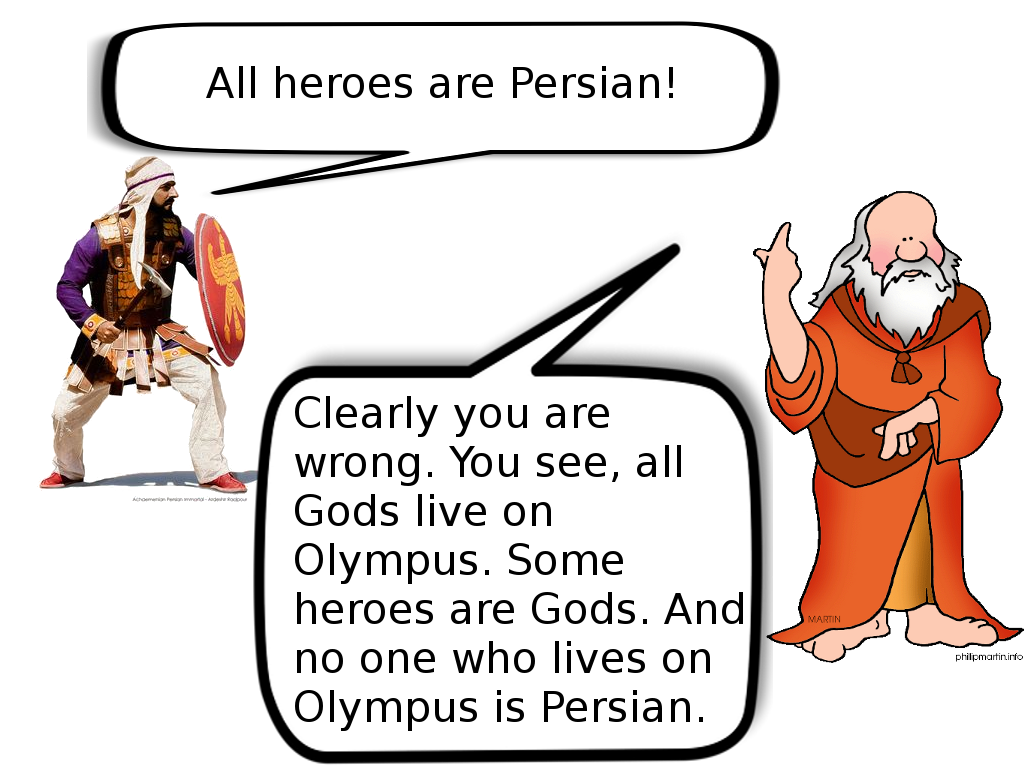
\includegraphics[height=7cm]{../img/persian_invaders.png}
\end{center}
\end{frame}

\begin{frame}[noframenumbering]{How Did You Solve This?}
\begin{center}
  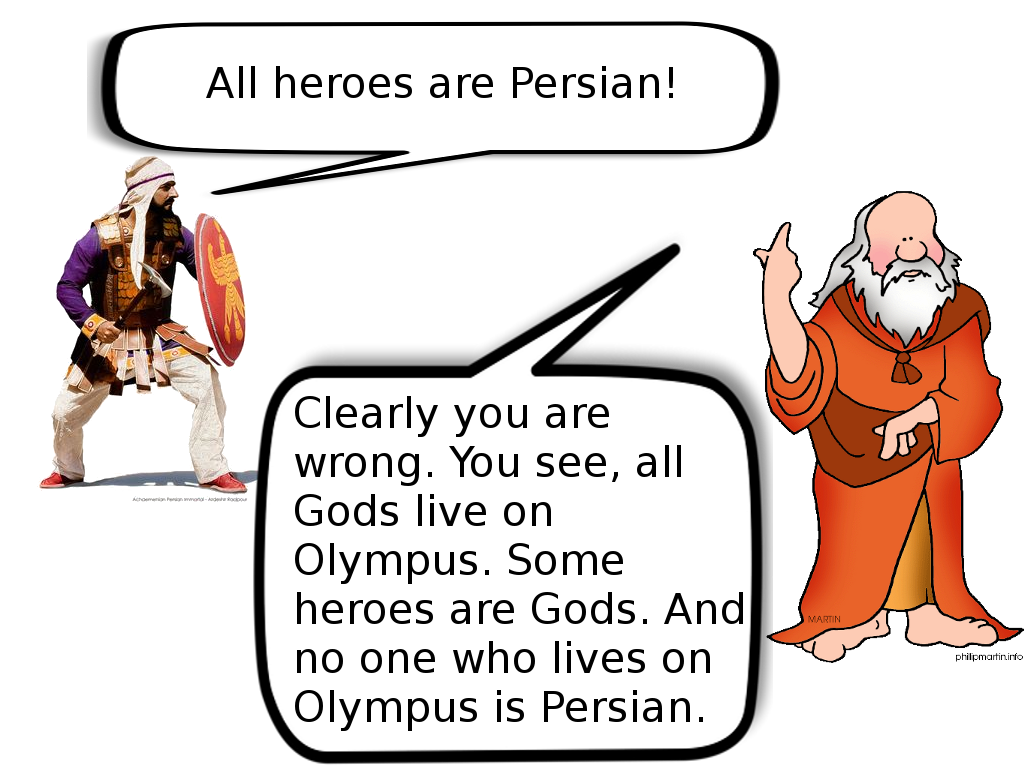
\includegraphics[height=7cm]{../img/persian_invaders.png}
\end{center}
\end{frame}

\begin{frame}[noframenumbering]{Show of Hands: First Order Logic?}
\begin{center}
\scalebox{0.5}{
$
\begin{nd}
\hypo {1} {\forall x~~\textrm{God}(x) \supset \textrm{LivesOnOlympus}(x)}
\hypo {2} {\exists x~~\textrm{Hero}(x) \land \textrm{God}(x)}
\hypo {3} {\lnot \exists x~~\textrm{LivesOnOlympus}(x) \land \textrm{Persian}(x)}

\open
  \hypo {4} {\forall x~~\textrm{Hero(x)} \supset \textrm{Persian}(x)}
  \open[a]
    \hypo {5}  {\textrm{Hero}(a) \land \textrm{God}(a)}                          \Ee{2}
    \have {6}  {\textrm{Hero}(a)}                                                \ae{5}
    \have {7}  {\textrm{Hero(a)} \supset \textrm{Persian}(a)}                    \Ae{4}
    \have {8}  {\textrm{Persian}(a)}                                             \ie{6,7}
    \have {9}  {\textrm{God}(a)}                                                 \ae{5}
    \have {10} {\textrm{God}(a) \supset \textrm{LivesOnOlympus}(a)}              \Ae{1}
    \have {11} {\textrm{LivesOnOlympus}(a)}                                      \ie{9,10}
    \have {12} {\textrm{LivesOnOlympus}(a) \land \textrm{Persian}(a)}            \ai{8,11} 
    \have {13} {\exists x~~\textrm{LivesOnOlympus}(x) \land \textrm{Persian}(x)} \Ei{12} 
  \close
  \have {14} {\exists x~~\textrm{LivesOnOlympus}(x) \land \textrm{Persian}(x)}   \r{12} 
  \have {15} {\bot}                                                              \by{$\bot$ I}{3,14}
\close
\have {16} {\lnot~~\forall x~~\textrm{Hero(x)} \supset \textrm{Persian}(x) }     \by{$\lnot$ I}{4--15}
\end{nd}
$
}
\end{center}
\end{frame}

%%%%%%%%%%%%%%%%%%% 
% SYLLOGISMS
%%%%%%%%%%%%%%%%%%%
\begin{frame}{Syllogisms: The First Natural Logic}
\begin{center}
\scalebox{0.5}{
  $
  \begin{nd}
  \hypo {1} {\ww{All Gods live on Mount Olympus}}
  \hypo {2} {\ww{Some heroes are Gods}}
  \hypo {3} {\ww{Nobody who lives on Mount Olympus is Persian}}
  \have {4} {\ww{Some heroes live on Mount Olympus}}  \by{AII (Darii)}{1,2}
  \have {5} {\ww{Some heroes are not Persian}}        \by{EIO (Ferio)}{4,3}
  \have {6} {\lnot~~\ww{All heroes are Persian}}      \by{SaP $\bot$ SoP}{5}
  \end{nd}
  $
}
\end{center}
\vspace{2ex}
\pause

%\hh{Syllogisms have some nice properties}
%\begin{itemize}
%  \item More cognitively grounded
%  \item Computationally efficient
%  \item \textbf{Uses only the syntax of natural language}
%\end{itemize}
%\vspace{2ex}
%\pause

\hh{...But syllogisms are cripplingly unexpressive}

\end{frame}

%%%%%%%%%%%%%%%%%%%% 
%% LOGIC AS BLACK BOX
%%%%%%%%%%%%%%%%%%%%
%\begin{frame}{Language Interpretation is a Black Box}
%\begin{tabular}{m{4cm} m{0.1cm} m{2.25cm} m{0.1cm} m{1cm}}
%  \w{All heroes are Persian} & $\Rightarrow$ & 
%    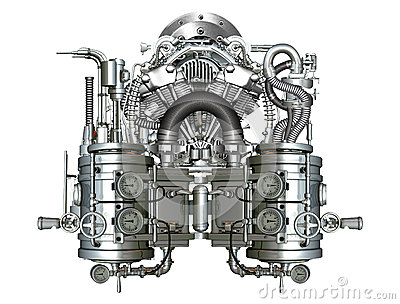
\includegraphics[height=2cm]{../img/complicated_machine.jpg} &
%    $\Rightarrow$ & $\{ true, false \}$ \\
%   \pause
%  
%  \w{All heroes are Persian} & $\Rightarrow$ & 
%    \hspace{1cm} $f$ & 
%    $\Rightarrow$ & $\{ true, false \}$
%\end{tabular}
%\pause
%\vspace{4ex}
%
%\hh{First Order Logic:} Evaluate $f$ in terms of predicates/connectives/etc. \\
%\vspace{2ex}
%\hh{Natural Logic:} What can we say about $f$ without evaluating it?
%\end{frame}
%
%%%%%%%%%%%%%%%%%%%% 
%% LOGIC AS BLACK BOX
%%%%%%%%%%%%%%%%%%%%
%\begin{frame}{Syllogisms: Invariants in $f$}
%\vspace{-4ex}
%\begin{center}
%\[ f(\w{All $x$ $y$}) \land f(\w{Some $z$ are $x$}) \vDash f(\w{Some $z$ $y$}) \]
%\[ f(\w{Some $z$ $y$}) \land f(\w{No $y$ are $q$}) \vDash f(\w{Some $z$ are not $q$}) \]
%\end{center}
%\vspace{2ex}
%
%\hh{Pattern matching $\Rightarrow$ Don't need to interpret $f$; $x$, $y$, $z$, $q$}
%\vspace{2ex}
%\pause
%
%\hh{Natural language proof theory:}
%\begin{center}
%\scalebox{0.5}{
%  $
%  \begin{nd}
%  \hypo {1} {\ww{All Gods live on Mount Olympus}}
%  \hypo {2} {\ww{Some heroes are Gods}}
%  \hypo {3} {\ww{Nobody who lives on Mount Olympus is Persian}}
%  \have {4} {\ww{Some heroes live on Mount Olympus}}  \by{AII (Darii)}{1,2}
%  \have {5} {\ww{Some heroes are not Persian}}        \by{EIO (Ferio)}{4,3}
%  \have {6} {\lnot~~\ww{All heroes are Persian}}      \by{SaP $\bot$ SoP}{5}
%  \end{nd}
%  $
%}
%\end{center}
%\end{frame}


%%%%%%%%%%%%%%%%%%% 
% MONOTONICITY IN ALGEBRA
%%%%%%%%%%%%%%%%%%%
\begin{frame}{Beyond Syllogisms: Monotonicity Calculus}
\begin{center}
  $f : X \rightarrow Y$ is \textit{monotone} w.r.t. partial orders 
    $\leq_X$, $\leq_Y~~$ 
    iff
    $~~\forall x_0 \forall x_1 \geq_X x_0; ~~ f(x_1) \geq_Y f(x_0)$. \\
\end{center}
\begin{center}
  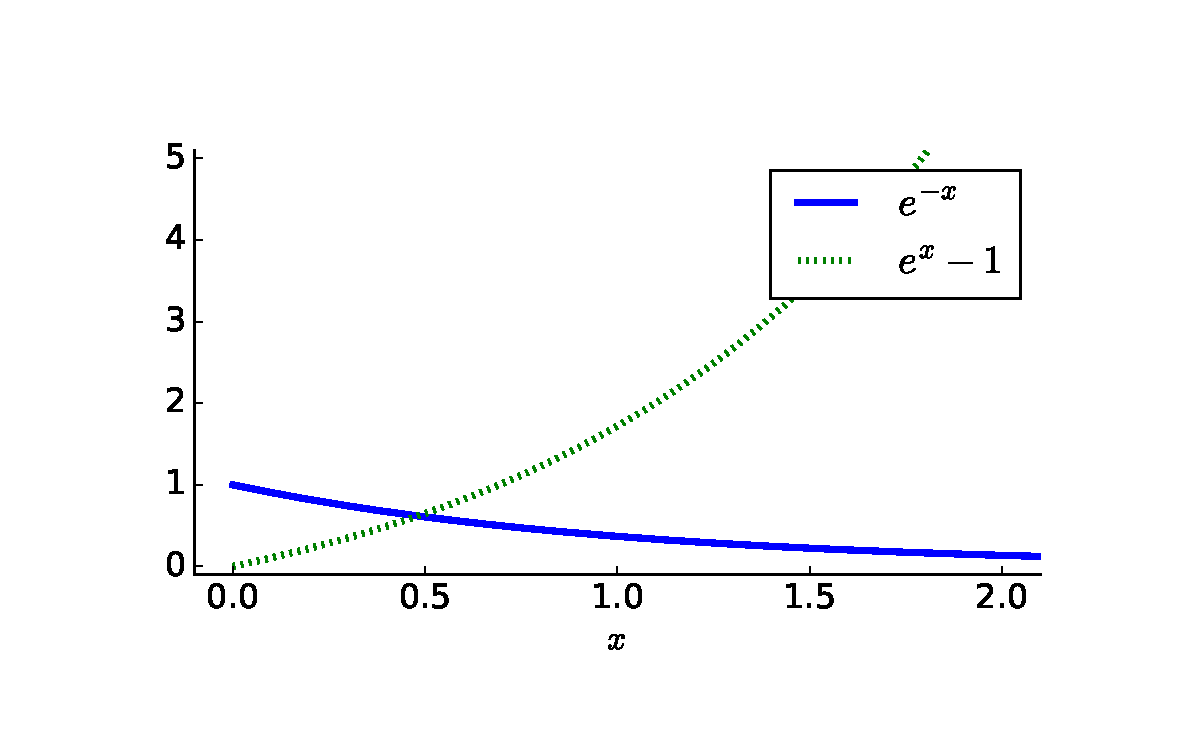
\includegraphics[height=5.5cm]{../img/monotonicity_math.pdf}
\end{center}
\footnotetext<.->{\cite{key:1991valencia-natlog,key:2014icard-natlog}}
\end{frame}



%%%%%%%%%%%%%%%%%%% 
% MONOTONICITY IN LANGUAGE (<_Y)
%%%%%%%%%%%%%%%%%%%
\begin{frame}{Monotonicity Calculus}
\begin{center}
  $f : X \rightarrow 
    \textcolor<2>{darkred}{Y}$ 
    is \textit{monotone} w.r.t. partial orders 
    $\leq_X$, \textcolor<2>{darkred}{$\leq_Y~~$} 
    iff
    $~~\forall x_0 \forall x_1 \geq_X x_0; ~~ f(x_1) \geq_Y f(x_0)$. \\
  \vspace{1ex}
  \hh{$f :$ denotations $\rightarrow$ truth values}
\end{center}

\pause
\vspace{1ex}

\hh{$\leq_Y$ for truth values}:
\begin{center}
\begin{tabular}{ll|cc}
\textbf{P} & \textbf{Q} & \textbf{P $\leq_Y$ Q} & \textcolor<2>{white}{\textbf{P $\supset$ Q}}  \\
true  & true  & \darkgreen{true}  & \darkgreen{\textcolor<2>{white}{true}} \\
true  & false & \darkred{false}   & \darkred{\textcolor<2>{white}{false}} \\
false & true  & \darkgreen{true}  & \darkgreen{\textcolor<2>{white}{true}} \\
false & false & \darkgreen{true}  & \darkgreen{\textcolor<2>{white}{true}}  
\end{tabular}
\end{center}
\pause
\vspace{1ex}

\begin{center}
  \hh{$\leq_Y$ denotes entailment}
\end{center}
\end{frame}

%%%%%%%%%%%%%%%%%%% 
% MONOTONICITY IN LANGUAGE (<_Y)
%%%%%%%%%%%%%%%%%%%
\begin{frame}[noframenumbering]{Monotonicity in Language}
\begin{center}
  $f : X \rightarrow Y$ 
    is \textit{monotone} w.r.t. partial orders 
    $\leq_X$, $\leq_Y~~$
    iff
    $~~\forall x_0 \forall x_1 \geq_X x_0; ~~ f(x_1) \geq_Y f(x_0)$. \\
  \vspace{1ex}
  \hh{$f :$ denotations $\rightarrow$ truth values}
\end{center}

\vspace{1ex}

\hh{$\leq_X$ for denotations}: subset.
  
\begin{center}
\begin{tabular}{ccc}
  \begin{tikzpicture}
    \def\vennB{(0.2,-0.2) circle (0.5)}
    \draw \vennB node [below] {};
    \begin{scope}
      \fill[fill=light] \vennB;
    \end{scope}
    \frameVenn
  \end{tikzpicture} & &
  
  \begin{tikzpicture}
    \def\vennB{(0.1,-0.1) circle (0.7)}
    \draw \vennB node [below] {};
    \begin{scope}
      \fill[fill=dark] \vennB;
    \end{scope}
    \frameVenn
  \end{tikzpicture} \\

  \denote{cat} & $\subseteq$ & \denote{feline}
\end{tabular}
\end{center}
\end{frame}


%%%%%%%%%%%%%%%%%%% 
% POLARITY
%%%%%%%%%%%%%%%%%%%
\def\title{Proofs in Natural Logic}
\def\header{
  \hh{Quantifiers are functions with monotonicity.} \\
  \vspace{2ex}
  \hh{Words are in either upward, downward, or non-monotone contexts.} \\
  \vspace{2ex}
}
\def\blurb{
  \hh{\textit{Polarity} is the direction a lexical item can ``move.'' } \\
}

\begin{frame}{\title}
  \header
  \pause
  \blurb
  \begin{center}
    \monoHeader
      \node[black]{animal};
      \node[black]{feline};
      \node[punktchain,color=blue]{cat};
      \node[black]{house cat};
    \end{tikzpicture}
  \end{center}
\end{frame}

\begin{frame}[noframenumbering]{\title}
  \header
  \blurb
  \begin{center}
    \monoUp{house cat}{cat}{feline}{animal}
  \end{center}
\end{frame}

\begin{frame}[noframenumbering]{\title}
  \header
  \blurb
  \begin{center}
    \monoUp{cat}{feline}{animal}{living thing}
  \end{center}
\end{frame}

\begin{frame}[noframenumbering]{\title}
  \header
  \blurb
  \begin{center}
    \monoUp{feline}{animal}{living thing}{thing}
  \end{center}
\end{frame}

\begin{frame}[noframenumbering]{\title}
  \header
  \blurb
  \begin{center}
    \monoDown{feline}{animal}{living thing}{thing}
  \end{center}
\end{frame}

\begin{frame}[noframenumbering]{\title}
  \header
  \blurb
  \begin{center}
    \monoDown{cat}{feline}{animal}{living thing}
  \end{center}
\end{frame}

\begin{frame}[noframenumbering]{\title}
  \header
  \blurb
  \begin{center}
    \monoDown{house cat}{cat}{feline}{animal}
  \end{center}
\end{frame}

%%%%%%%%%%%%%%%%%%% 
% NATLOG ANIMATION
%%%%%%%%%%%%%%%%%%%
\input example.tex
	

%%%%%%%%%%%%%%%%%%% 
% REASONING WITH EXCLUSION
%%%%%%%%%%%%%%%%%%%
\begin{frame}{Reasoning with Negation (Exclusion)}
\begin{center}
\begin{tabular}{ccc}
\forwardVenn & \reverseVenn & \equivalentVenn \\
\pause
\negateVenn & \alternateVenn & \coverVenn
\end{tabular}
\end{center}
\footnotetext<.->{\cite{key:2008maccartney-natlog}}
\end{frame}


%%%%%%%%%%%%%%%%%%% 
% TRANSITIVITY
%%%%%%%%%%%%%%%%%%%
\def\title{``Join Table''}
\begin{frame}{\title}
\begin{center}
	\begin{tabular}{|c||c|c|c|c|c|c|c|}
    \hline
    $\bowtie$ & $\equivalent$ & $\forward$ & $\reverse$ & $\negate$ & $\alternate$ & $\cover$ & $\independent$ \\
    \hline
    $\equivalent$ & $\equivalent$ & $\forward$ & $\reverse$ & $\negate$ & $\alternate$ & $\cover$ & $\independent$ \\
    $\forward$ & $\forward$ & $\forward$ & $\independent$ & $\alternate$ & $\alternate$ & $\independent$ & $\independent$ \\
    $\reverse$ & $\reverse$ & $\independent$ & $\reverse$ & $\cover$ & $\independent$ & $\cover$ & $\independent$  \\
    $\negate$ & $\negate$ & $\cover$ & $\alternate$ & $\equivalent$ & $\reverse$ & $\forward$ & $\independent$  \\
    $\alternate$ & $\alternate$ & $\independent$ & $\alternate$ & $\forward$ & $\independent$ & $\forward$ & $\independent$  \\
    $\cover$ & $\cover$ & $\cover$ & $\independent$ & $\reverse$ & $\reverse$ & $\independent$ & $\independent$  \\
    $\independent$ & $\independent$ & $\independent$ & $\independent$ & $\independent$ & $\independent$ & $\independent$ & $\independent$ \\
    \hline
	\end{tabular}
\end{center}
\end{frame}

%%%%%%%%%%%%%%%%%%% 
% TRANSITIVITY
%%%%%%%%%%%%%%%%%%%
\def\title{Contribution: Don't Need Join Table}
\begin{frame}[noframenumbering]{\title}
\begin{center}
  \scalebox{0.85}{\completeFSA}
\end{center}
\footnotetext<.->{\cite{key:2014angeli-naturalli}}
\end{frame}


\begin{frame}[noframenumbering]{\title}
\begin{center}
  \scalebox{0.85}{\collapsedFSA}
\end{center}
\footnotetext<.->{\cite{key:2014angeli-naturalli}}
\end{frame}


%%%%%%%%%%%%%%%%%%%% 
%% MONOTONICITY CALCULUS
%%%%%%%%%%%%%%%%%%%%
%\def\title{Monotonicity Calculus}
%\begin{frame}{\title}
%\begin{center}
%\hh{Does a given mutation to a sentence preserve its truth?}
%\end{center}
%\vspace{1em}
%\pause
%
%\hh{Logic over natural language}
%\begin{itemize}
%\item \textit{Instantaneous} and \textit{perfect} semantic parsing!
%\item Plays nice with lexical methods
%\end{itemize}
%\vspace{1ex}
%\pause
%
%\hh{Tractable}
%\begin{itemize}
%\item Polynomial time entailment checking \cite{key:2008maccartney-natlog}.
%\end{itemize}
%\vspace{1ex}
%\pause
%
%\hh{Expressive (for common inferences)}
%\begin{itemize}
%\item Second-order phenomena; \w{most}; quantifier scoping
%\pause
%\item No free lunch: shallow quantification; single-premise only
%\end{itemize}
%\footnotetext<.->{\cite{key:1991valencia-natlog,key:2008maccartney-natlog,key:2014icard-natlog}}
%\end{frame}
%
%
%%%%%%%%%%%%%%%%%%%%%%%%%%%%%%%%%%%%%%%%%%%%%%%%%%%%%%%%%%%%%%%%%%%%%%%%%%%%%%%%
%% INFERENCE
%%%%%%%%%%%%%%%%%%%%%%%%%%%%%%%%%%%%%%%%%%%%%%%%%%%%%%%%%%%%%%%%%%%%%%%%%%%%%%%%
%
%
%%%%%%%%%%%%%%%%%%%% 
%% REMINDER
%%%%%%%%%%%%%%%%%%%%
%\begin{frame}[noframenumbering]{Problem Setup}
%\begin{center}
%  \teaserFullDerivation
%\end{center}
%\end{frame}

%%%%%%%%%%%%%%%%%% 
% EXAMPLE SEARCH
%%%%%%%%%%%%%%%%%%
\def\title{An Example Search}
\def\eat{\monoDownR{slurp}{eat}{consume}{}}
\begin{frame}{\title}
  \begin{center}
    \hh{Shorthand for a node:} \\
    \vspace{0.5cm}
    \scalebox{0.75}{\no \carnivores \eat \animals} \\
    \vspace{0.5cm}
    
\includegraphics[height=2.0cm]{../img/dArrow.jpg} \\
    \vspace{0,5cm}
      \setstyles
      \begin{tikzpicture}[grow=down, sloped]
      \node[boxfact](main) {\w{No carnivores eat animals?}};
      \end{tikzpicture}
  \end{center}
\end{frame}

\input exampleSearch2pane.tex
\input exampleSearchEdges.tex

%%%%%%%%%%%%%%%%%%% 
% EDGE TEMPLATES
%%%%%%%%%%%%%%%%%%%
\begin{frame}{Edge Templates}
\begin{center}
  \begin{tabular}{p{0.4\textwidth}p{0.20\textwidth}}
    \multicolumn{1}{c}{\textbf{Template}} & \multicolumn{1}{c}{\textbf{Instance}} \\
    Hypernym & \w{animal} $\rightarrow$ \w{cat} \\
    Hyponym  & \w{cat} $\rightarrow$ \w{animal} \\
    Antonym  & \w{good} $\rightarrow$ \w{bad} \\
    Synonym  & \w{cat} $\rightarrow$ \w{true cat} \\
    & \\
    Add Word  & \w{cat} $\rightarrow$ \w{$\cdot$} \\
    Delete Word  & $\cdot$ $\rightarrow$ \w{cat} \\
    & \\
    Operator Weaken & \w{some} $\rightarrow$ \w{all} \\
    Operator Strengthen & \w{all} $\rightarrow$ \w{some} \\
    Operator Negate & \w{all} $\rightarrow$ \w{no} \\
    Operator Synonym & \w{all} $\rightarrow$ \w{every} \\
    & \\
    Nearest Neighbor  & \w{cat} $\rightarrow$ \w{dog} \\
  \end{tabular}
\end{center}
\end{frame}


%%%%%%%%%%%%%%%%%%% 
% SOFT LOGIC
%%%%%%%%%%%%%%%%%%%
\begin{frame}{``Soft'' Natural Logic}
\hh{Want to make likely (but not certain) inferences}.
\begin{itemize}
  \item Same motivation as Markov Logic, Probabilistic Soft Logic, etc.
  \pause
  \item Each \textit{edge template} has a cost $\theta \geq 0$.
\end{itemize}
\vspace{0.5cm}
\pause

\hh{Detail:} Variation among \textit{edge instances} of a template.
\begin{itemize}
  \item WordNet: \w{cat} $\rightarrow$ \w{feline} \textbf{vs.} \w{cup} $\rightarrow$ \w{container}.
  \item Nearest neighbors distance.
  \item Each \textit{edge instance} has a distance $f$.
\end{itemize}
\vspace{0.5cm}
\pause

\begin{tabular}{ll}
\hh{Cost of an edge is} & $\theta_i \cdot f_i$. \\
\pause
\hh{Cost of a path is} & $\theta \cdot \mathbf{f}$. \pause \\
\multicolumn{2}{l}{\hh{Can learn parameters $\theta$}.}
\end{tabular}

\end{frame}


%%%%%%%%%%%%%%%%%%%%%%%%%%%%%%%%%%%%%%%%%%%%%%%%%%%%%%%%%%%%%%%%%%%%%%%%%%%%%%%
% RESULTS
%%%%%%%%%%%%%%%%%%%%%%%%%%%%%%%%%%%%%%%%%%%%%%%%%%%%%%%%%%%%%%%%%%%%%%%%%%%%%%%

%%%%%%%%%%%%%%%%%%% 
% ConceptNet INTRO
%%%%%%%%%%%%%%%%%%%
\begin{frame}{Experiments}
\hh{ConceptNet:}
\begin{itemize}
  \item A semi-curated collection of common-sense facts. \\
    \vspace{0.1cm}
    \true{not all birds can fly} \\
    \true{noses are used to smell} \\
    \true{nobody wants to die} \\
    \true{music is used for pleasure}
    \vspace{0.1cm}
  \item Negatives: ReVerb extractions marked false by Turkers.
  \item Small (1378 train / 1080 test), but fairly broad coverage.
\end{itemize}
\vspace{0.5cm}
\pause

\hh{Our Knowledge Base:}
\begin{itemize}
  \item 270 million lemmatized Ollie extractions.
\end{itemize}
\end{frame}
  
%%%%%%%%%%%%%%%%%%% 
% ConceptNet RESULTS
%%%%%%%%%%%%%%%%%%%
\begin{frame}{ConceptNet Results}
\hh{Systems}
\begin{itemize}
  \item[] \textbf{Direct Lookup}: Lookup by lemmas.
  \item[] \textbf{This Work}.
  \pause
  \item[] \textbf{This Work - Lookup}: Remove query facts from KB.
\end{itemize}
\pause

\begin{center}
  \begin{tabular}{lcc}
    System             & P     & R    \\
    \hline
    Direct Lookup      & 100.0 & \textbf<5-5>{12.1} \\
    \pause
    This Work          & 90.6  & \textbf<5-5>{49.1} \\
    This Work - Lookup & 88.8  & 40.1 \\
  \end{tabular}
\end{center}
\pause

\begin{itemize}
  \item 4x improvement in recall.
\end{itemize}
\end{frame}


\begin{frame}{New Solutions to Old Problems}
\hh{Old Problem:} Dozens of clever meaning representations for language. \\
\vspace{1ex}
\pause
\hh{New Solution:} Treat text as the meaning representation!
\vspace{4ex}
\pause

\hh{Old Problem:} Collect ontologies of true facts.
\begin{center}
\begin{tabular}{ccc}
  
\includegraphics[height=1cm]{../img/cyc.png} & 
  
\includegraphics[height=1cm]{../img/freebase-logo.jpg} & 
  
\includegraphics[height=1cm]{../img/conceptnet.png}
\end{tabular}
\end{center}
\pause
\hh{New Solution:} Treat unstructured text as your ontology! \\
\vspace{2ex}


\end{frame}
